\documentclass[acmtog,review,anonymous]{acmart}

\usepackage{booktabs} % For formal tables
\usepackage{subcaption}

\DeclareMathOperator{\sinc}{sinc}
\DeclareMathOperator{\rect}{rect}


\usepackage[ruled]{algorithm2e} % For algorithms
\renewcommand{\algorithmcfname}{ALGORITHM}
\SetAlFnt{\small}
\SetAlCapFnt{\small}
\SetAlCapNameFnt{\small}
\SetAlCapHSkip{0pt}
\IncMargin{-\parindent}

% Metadata Information
\acmJournal{TOG}
\acmVolume{9}
\acmNumber{4}
\acmArticle{39}
\acmYear{2010}
\acmMonth{3}

% Copyright
\setcopyright{none}
%\setcopyright{acmcopyright}
%\setcopyright{acmlicensed}
%\setcopyright{rightsretained}
%\setcopyright{usgov}
%\setcopyright{usgovmixed}
%\setcopyright{cagov}
%\setcopyright{cagovmixed}

% DOI
\acmDOI{0000001.0000001_2}

% use the "authoryear" citation style.
\citestyle{acmauthoryear}
\setcitestyle{square}

% Document starts
\begin{document}
% Title portion
\title{Near-eye Dual-layer Light Field Display}

\author{Rafael Romeiro}
\affiliation{%
  \institution{Universidade Federal do Rio de Janeiro}
  \streetaddress{Cidade Universitária — Ilha do Fundão, Caixa Postal 68530}
  \city{Rio de Janeiro}
  \state{RJ}
  \postcode{21945-970}
}
\email{romeiro@cos.ufrj.br}

\author{Ricardo Marroquim}
\affiliation{%
  \institution{Universidade Federal do Rio de Janeiro}
  \streetaddress{Cidade Universitária — Ilha do Fundão, Caixa Postal 68530}
  \city{Rio de Janeiro}
  \state{RJ}
  \postcode{21945-970}
}
\email{marroquim@cos.ufrj.br}

% The default list of authors is too long for headers}
\renewcommand{\shortauthors}{R. Romeiro et. al.}

\begin{abstract}
Abstract...
\end{abstract}


%
% The code below should be generated by the tool at
% http://dl.acm.org/ccs.cfm
% Please copy and paste the code instead of the example below.
%
\begin{CCSXML}
<ccs2012>
 <concept>
  <concept_id>10010520.10010553.10010562</concept_id>
  <concept_desc>Computer systems organization~Embedded systems</concept_desc>
  <concept_significance>500</concept_significance>
 </concept>
 <concept>
  <concept_id>10010520.10010575.10010755</concept_id>
  <concept_desc>Computer systems organization~Redundancy</concept_desc>
  <concept_significance>300</concept_significance>
 </concept>
 <concept>
  <concept_id>10010520.10010553.10010554</concept_id>
  <concept_desc>Computer systems organization~Robotics</concept_desc>
  <concept_significance>100</concept_significance>
 </concept>
 <concept>
  <concept_id>10003033.10003083.10003095</concept_id>
  <concept_desc>Networks~Network reliability</concept_desc>
  <concept_significance>100</concept_significance>
 </concept>
</ccs2012>
\end{CCSXML}

\ccsdesc[500]{Computer systems organization~Embedded systems}
\ccsdesc[300]{Computer systems organization~Redundancy}
\ccsdesc{Computer systems organization~Robotics}
\ccsdesc[100]{Networks~Network reliability}

%
% End generated code
%

% We no longer use \terms command
%\terms{Design, Algorithms, Performance}

\keywords{ACM proceedings, \LaTeX, text tagging}


\thanks{This work is supported by CAPES.}

\maketitle

\section{Introduction}

Introduction...

\subsection{Contributions}

This paper makes the following contributions:

\textbf{Contribution 1.} Description of contribution 1.

\textbf{Contribution 2.} Description of contribution 2.

\section{Spectral analysis}

\subsection{Light field representation}

The radiance of a light ray in 3d space at the position $(x, y, z)$ and direction $(u, v)$ can be represented by the plenoptic function $P(x, y, z, u, v)$. Following \cite{Chai:2000:PS:344779.344932}, the coordinates $(u, v)$ are taken as the intersection of the ray with a plane orthogonal to the $z$ direction at unit distance relative to $(x, y, z)$ as depicted in figure \ref{fig:plenoptic}.

The canonical 4d light field $L(x, y, u, v) = P(x, y, 0, u, v)$ describes the radiance reaching the plane $z = 0$. The values in $L(x, y, u, v)$ can be propagated to another plane at $z = z_{local}$ and define a local light field $L_{local}(x, y, u, v)$. Note that $L_{local}(x, y, u, v)$ is different from $P(x, y, z_{local}, u, v)$ due to occlusions and is described only by the radiance along rays in empty space reaching the plane $z = 0$.

We refer to $(x, y)$ as \emph{spatial} coordinates and to $(u, v)$ as \emph{angular} coordinates. Throughout this work we address a 2d spatio-angular slice of the light field, $L(x, u)$. The extension to the full 4d light field is mostly straightforward and any difference will be indicated whenever necessary.

As shown in figure \ref{fig:local}, a local light field relates to the canonical light field by $L_{local}(x, u) = L(x - uz_{local}, u)$ or, in matrix representation, by eq. \ref{eq:local}.

\begin{equation} \label{eq:local}
L_{local}\left(\begin{bmatrix}x\\u\end{bmatrix}\right) =
L\left(\begin{bmatrix}1 && -z_{local}\\0 && 1\end{bmatrix} \begin{bmatrix}x\\u\end{bmatrix}\right)
\end{equation}

We denote the spatial and angular frequencies as $\omega_{x}$ and $\omega_{u}$, respectively. The local light field spectrum $\hat{L}_{local}(\omega_{x}, \omega_{u})$ can then be described from the canonical light field spectrum $\hat{L}(\omega_{x}, \omega_{u})$ (eq. \ref{eq:strech}).

\begin{equation} \label{eq:strech}
\hat{L}_{local}\left(\begin{bmatrix}\omega_{x}\\\omega_{u}\end{bmatrix}\right) =
\hat{L}\left(\begin{bmatrix}1 && 0\\z_{local} && 1\end{bmatrix} \begin{bmatrix}\omega_{x}\\\omega_{u}\end{bmatrix}\right)
\end{equation}

\subsection{Perceived image spectrum}

Images can be synthesized by selecting and combining rays from the light field. In this subsection we describe what an observer would see for a given light field reaching his pupil. Given the position and orientation of the observer, we choose to place the canonical light field over the pupil and orthogonal to the observer main optical axis (fig. \ref{eq:observer}).

We assume a thin lens camera model with the retina at $z_{r}$ and the pupil lens giving focus at an arbitrary distance $z_{f}$. The light field reaching the retina can be described by the local light field on the plane at focus (eq. \ref{eq:focus}). Using eq. \ref{eq:local} and eq. \ref{eq:focus}, the retina light field can be described by the light field reaching the pupil (eq. \ref{eq:pupil}).

\begin{equation} \label{eq:focus}
L_{r}\left(\begin{bmatrix}x\\u\end{bmatrix}\right) =
L_{f}\left(\begin{bmatrix}\frac{z_{f}}{z_{r}} && 0\\\frac{1}{z_{r}} - \frac{1}{z_{f}} && \frac{z_{r}}{z_{f}}\end{bmatrix} \begin{bmatrix}x\\u\end{bmatrix}\right)
\end{equation}

\begin{equation} \label{eq:pupil}
L_{r}\left(\begin{bmatrix}x\\u\end{bmatrix}\right) =
L_{p}\left(\begin{bmatrix}1 && -z_{r}\\\frac{1}{z_{r}} - \frac{1}{z_{f}} && \frac{z_{r}}{z_{f}}\end{bmatrix} \begin{bmatrix}x\\u\end{bmatrix}\right)
\end{equation}

The pupil light field is equal to the canonical light field with the rays outside of the pupil aperture being blocked, viz., $L_{p}(x, u) = L(x, u) \rect(\frac{x}{a})$. Where $a$ is the pupil aperture diameter and $\rect(x) = 1$ for $|x| < 0.5$ and $0$ otherwise. Finaly, the retina light field can be described by the canonical light field (eq. \ref{eq:canon}).

\begin{equation} \label{eq:canon}
L_{r}\left(\begin{bmatrix}x\\u\end{bmatrix}\right) =
L\left(\begin{bmatrix}1 && -z_{r}\\\frac{1}{z_{r}} - \frac{1}{z_{f}} && \frac{z_{r}}{z_{f}}\end{bmatrix} \begin{bmatrix}x\\u\end{bmatrix}\right)
\rect\left(\frac{x - u z_{r}}{a}\right)
\end{equation}

The image formed on the retina is given by the integration of the retina light field over the angular coordinate (eq. \ref{eq:image}). Applying eq. \ref{eq:image} inside the definition of the image spectrum we have eq. \ref{eq:imagespectrum}.

\begin{equation} \label{eq:image}
I(x) = \int_{-\infty}^{\infty} L_{r}\left(x, u\right) du
\end{equation}

\begin{equation} \label{eq:imagespectrum}
\begin{split}
\hat{I}(\omega_{x}) = \int_{-\infty}^{\infty} I(x) e^{-2 \pi i \omega_{x} x} dx =\\
=\iint_{-\infty}^{\infty} L_{r}\left(x, u\right) e^{-2 \pi i \omega_{x} x} dx du
\end{split}
\end{equation}

Given that the retina light field spectrum can be written, by definition, as in eq. \ref{eq:retinaspectrum}. Comparing eq. \ref{eq:imagespectrum} and eq. \ref{eq:retinaspectrum}, we can assert that $\hat{I}(\omega_{x}) = \hat{L}_{r}(\omega_{x}, 0)$.

\begin{equation} \label{eq:retinaspectrum}
\hat{L}_{r}(\omega_{x}, \omega_{u}) =
\iint_{-\infty}^{\infty} L_{r}\left(x, u\right) e^{-2 \pi i \omega_{x} x} e^{-2 \pi i \omega_{u} u} dx du
\end{equation}

From eq. \ref{eq:pupil}, the retina light field spectrum can be written as in eq. \ref{eq:retinaspectrum2} and thus the image spectrum can be written as in eq. \ref{eq:imagespectrum2}, where $\delta$ denotes the Dirac delta function and $\ast$ denotes the two dimensional convolution operation over $(\omega_{x}, \omega_{u})$.

\begin{equation} \label{eq:retinaspectrum2}
\hat{L}_{r}\left(\begin{bmatrix}\omega_{x}\\\omega_{u}\end{bmatrix}\right) =
\hat{L}_{p}\left(\begin{bmatrix}\frac{z_{r}}{z_{f}} && \frac{1}{z_{f}} - \frac{1}{z_{r}}\\z_{r} && 1\end{bmatrix} \begin{bmatrix}\omega_{x}\\\omega_{u}\end{bmatrix}\right)
\end{equation}

\begin{equation} \label{eq:imagespectrum2}
\begin{split}
\hat{I}(\omega_{x}) = \hat{L}_{r}\left(\begin{bmatrix}\omega_{x}\\0\end{bmatrix}\right) =
\hat{L}_{p}\left(\begin{bmatrix}\frac{z_{r}}{z_{f}}\omega_{x}\\z_{r}\omega_{x}\end{bmatrix}\right) =\\
= \hat{L}\left(\begin{bmatrix}\frac{z_{r}}{z_{f}}\omega_{x}\\z_{r}\omega_{x}\end{bmatrix}\right) \ast \left[ a \sinc\left(a \frac{z_{r}}{z_{f}} \omega_{x}\right) \delta(z_{r} \omega_{x}) \right]
\end{split}
\end{equation}

The final discrete image is a sampling of the continuous image signal formed on the retina. The maximum frequency $\xi_{x}$ which can be represented without aliasing is determined from the image sampling rate through Nyquist-Shannon theorem.

Regardless of the focus distance $z_{f}$, the maximum angular frequency on the canonical light field which can still be represented in the image without aliasing is $z_{r} \xi_{x}$. Therefore, when sampling the canonical light field for an observer (with unknown and possibly dynamic focus distance), one should not be concerned about capturing angular frequencies above $z_{r} \xi_{x}$.

Taking the full 4d light field into account, if the 2d retina image is sampled in a rectangular lattice (like a camera), then the non-vanishing intervals of horizontal and vertical spatial frequencies $(\omega_{x}, \omega_{y})$ are seperable and the 4d light field spectrum is the product of two separate spectra of 2d spatio-angular slices as described above. The maximum angular frequencies to be captured in the 4d canonical light field are $\omega_{u} = z_{r} \xi_{x}$ and $\omega_{v} = z_{r} \xi_{y}$.

On the other hand, if the 2d image is sampled in a hexagonal lattice (like the human eye), the image spectral support is not seperable and neither is the spectral support for the 4d canonical light field. Even so, the 4d canonical light field angular components are still bandlimited and independent of focus distance. In any case, an artificial rectangular spectral support containing the actual image spectrum can be assumed, allowing the light field spectrum to be seperable into two spatio-angular slices at the cost of higher sampling rates.

\subsection{Bounded Lambertian scene}

\section{Light field representation}

\begin{figure}[h]
  \centering
  \begin{subfigure}[t]{1in}
    \centering
    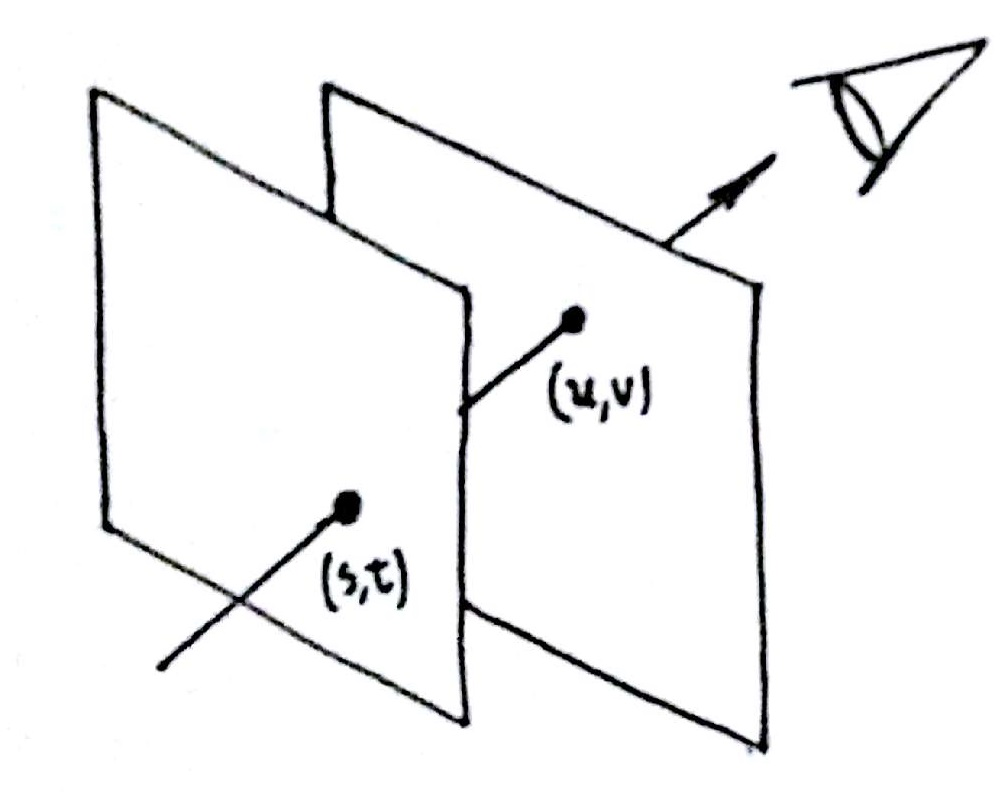
\includegraphics[width=1in]{figures/4dlf}
    \caption{4d light field}\label{fig:4dlf}
  \end{subfigure}
  \quad
  \begin{subfigure}[t]{1in}
    \centering
    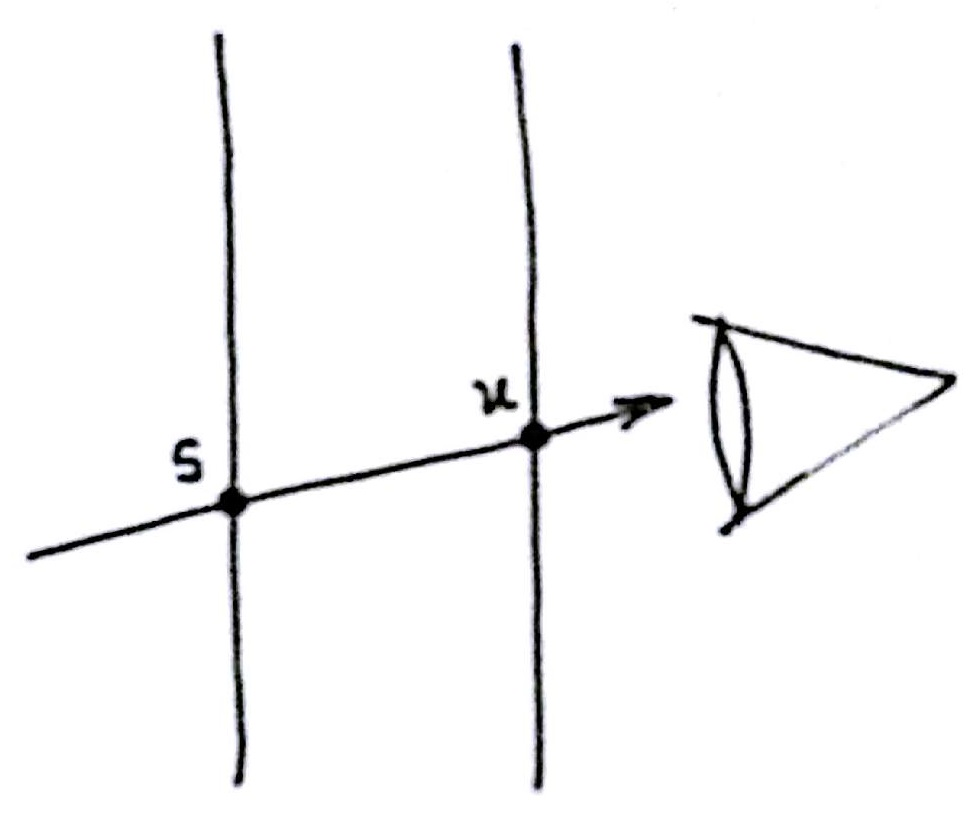
\includegraphics[width=1in]{figures/2dslice}
    \caption{2d slice}\label{fig:2dslice}
  \end{subfigure}
  \caption{Two-plane parameterization}\label{fig:globalparam}
\end{figure}

Following the notation in~\cite{Levoy:1996:LFR:237170.237199,Gortler:1996:LUM:237170.237200} we use the global two-plane parameterization. A light ray $l(s, t, u, v)$ is then defined by its intersections with two parallel planes (figure \ref{fig:4dlf}). We will refer to the coordinates on the plane closer to the observer as the \emph{angular} coordinates $(u, v)$ and on the farther as the \emph{spatial} coordinates $(s, t)$.

Throughout this work we address a 2d spatio-angular light field slice (figure \ref{fig:2dslice}). The extension to the full 4d light field is mostly straightforward and any difference will be indicated whenever necessary. Also, with no loss of generality, we assume the planes to be one unit apart.

\subsection{Local parameterization}

\begin{figure}[h]
  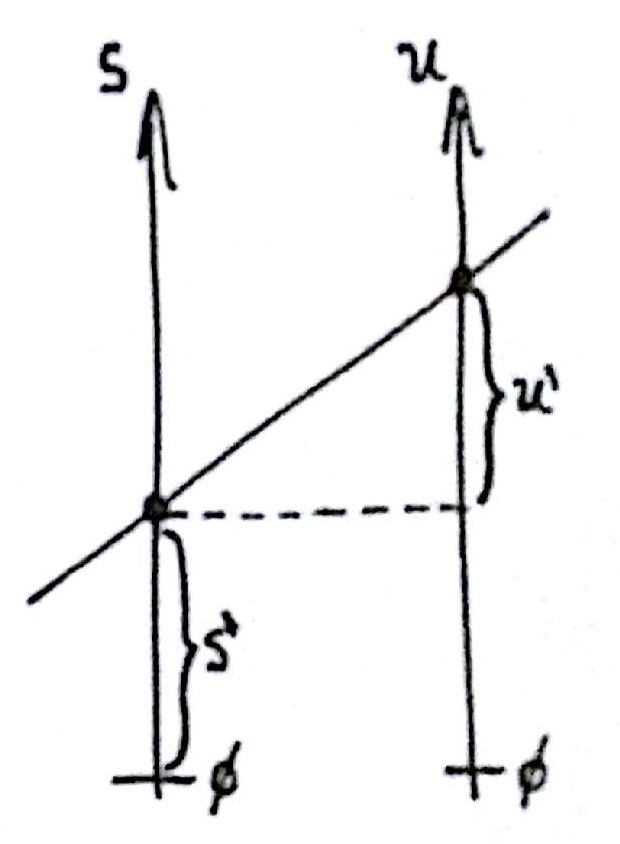
\includegraphics[width=1in]{figures/localparam}
  \caption{Relationship between global parameters $(s, u)$ and local parameters $(s', u')$}
  \label{fig:localparam}
\end{figure}

Some related works use a local two-plane parameterization\cite{Chai:2000:PS:344779.344932}. On those cases the spatial coordinates are absolute while the angular coordinates are taken relative to the spatial coordinates (figure \ref{fig:localparam}). This induces a shear on the angular coordinates when compared to the global parameterization, $l(s, t) = l(s', s' + u')$. Accordingly, on the frequency domain there will be a shear on the spatial components, $\hat{l}(\omega_{s}, \omega_{u}) = \hat{l}(\omega_{s'} - \omega_{u'}, \omega_{u'})$. Bearing this in mind, all conclusions remain the same with minor modifications. It is also important to notice that the terms spatial and angular (or directional) are sometimes swaped since their meanings are a matter of interpretation.

\section{Fourier spectrum analysis}

Many previous works analysed the light field spectrum for scenes with different levels of complexity\cite{Liang:2015:LTF:2742222.2665075,Chai:2000:PS:344779.344932,Durand:2005:FAL:1073204.1073320,Ng:2005:FSP:1073204.1073256}. In this section, we review the spectrum for a single Lambertian surface as well as for Lambertian scenes free of occlusions.

\subsection{Lambertian surface} \label{subsec:lambsurf}

Considering a surface parallel to the light field parameterization planes and at a distance $d$ from the angular plane (figure \ref{fig:lambsurf}), a ray intersects this surface on $x = ds + (1-d)u$. If the surface is Lambertian and $f(x)$ denotes the radiance of any ray passing through $x$, then $l(s, u) = f(ds + (1-d)u)$. Thus, the Fourier transform of the light field will be $\hat{l}(\omega_{s},\omega_{u}) = \hat{f}(\omega_{s}/d)\delta((1 - \frac{1}{d})\omega_{s} + \omega_{u})$. From this we can draw two important conclusions: The spectrum of the Lambertian surface lies in the line $\omega_{u} = (\frac{1}{d} - 1)\omega_{s}$ and $\omega_{s} = d\omega_{x}$.

\begin{figure}[h]
  \centering
  \begin{subfigure}[t]{1.1in}
    \centering
    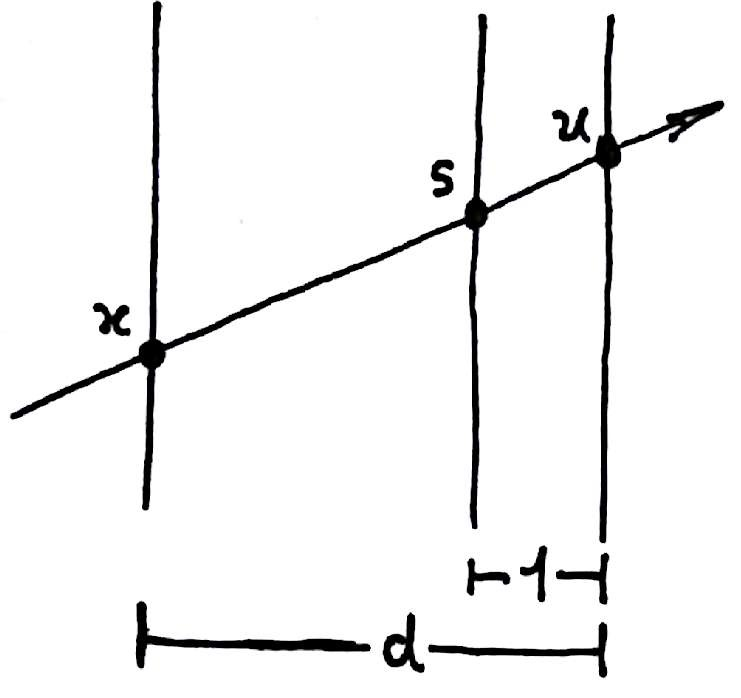
\includegraphics[height=1in]{figures/lambsurf}
    \caption{Surface at distance $d$}\label{fig:lambsurf}
  \end{subfigure}
  \quad
  \begin{subfigure}[t]{1in}
    \centering
    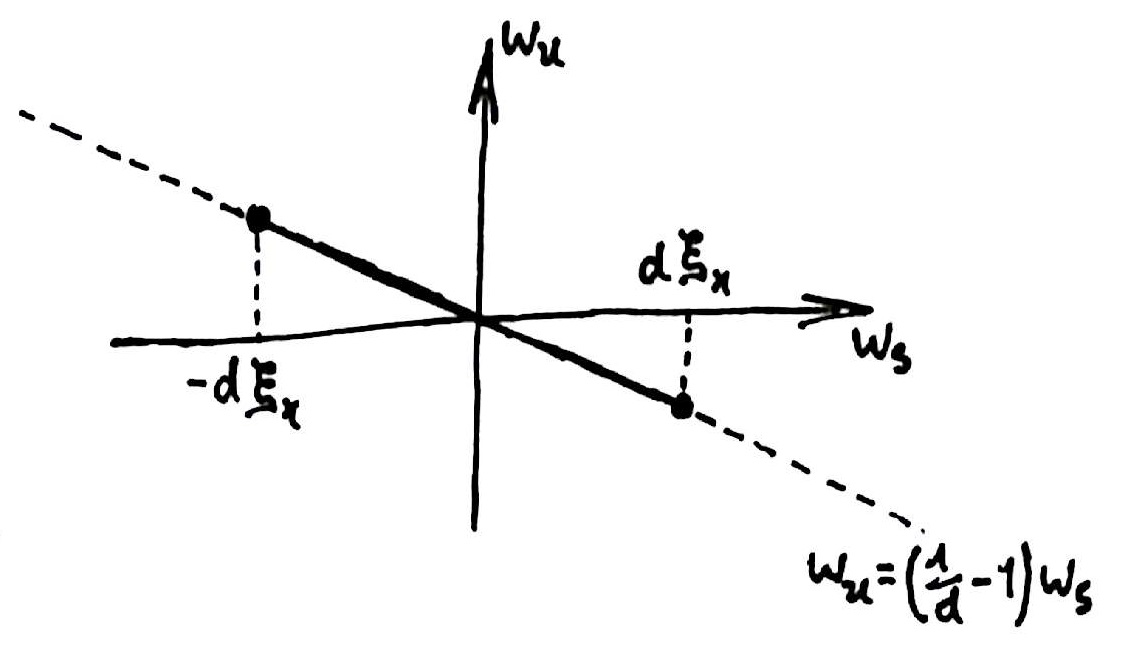
\includegraphics[height=1in]{figures/lambspec}
    \caption{Spectrum}\label{fig:lambspec}
  \end{subfigure}
  \caption{Single lambertian surface}
\end{figure}

Restricting the frequency $\omega_{x}$ on the surface makes the light field bandlimited. If the maximum frequency on the surface is $\xi_{x}$ then the light field spectrum becomes a line segment as shown in figure \ref{fig:lambspec}.

\subsection{Bounded scene} \label{subsec:scene}

A Lambertian scene between a maximum distance $d_{max}$ and minimum distance $d_{min}$ can be decomposed as infinite Lambertian surfaces stacked. Without taking visibility into account, the light field spectrum is bounded by the lines $\omega_{u} = (\frac{1}{d_{max}} - 1)\omega_{s}$ and $\omega_{u} = (\frac{1}{d_{min}} - 1)\omega_{s}$ (figure \ref{fig:scenespec}). Even though occlusions can introduce high frequencies\cite{Durand:2005:FAL:1073204.1073320}, this effect will be ignored as in \cite{Chai:2000:PS:344779.344932}.

\begin{figure}[h]
  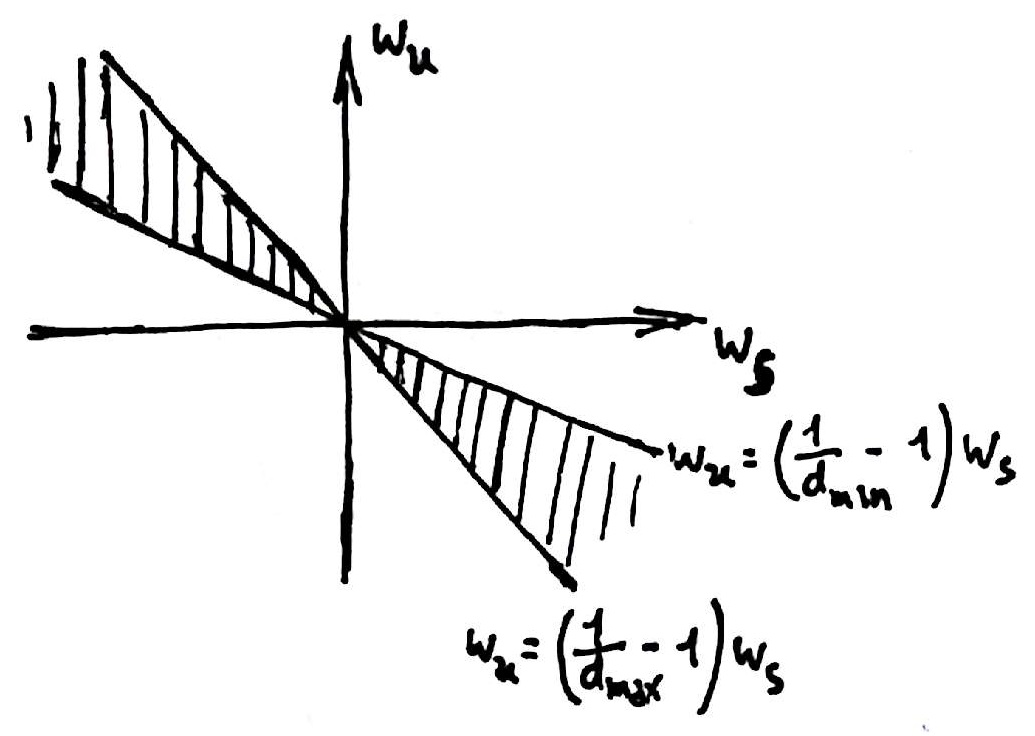
\includegraphics[height=1in]{figures/scenespec}
  \caption{Bounded scene spectrum}
  \label{fig:scenespec}
\end{figure}

\section{Rendering}

Images can be synthesized by selecting and combining rays from the light field. Assuming the position of the observer is known, we place the angular plane and the spatial plane at the distances $0$ and $1$ from it, respectively. Both planes are orthogonal to the observer main optical axis. Parallel to the parameterization planes will be the observer image plane, at a distance $d_{i}$ on the opposite direction (figure \ref{fig:observer}).

\begin{figure}[h]
  \centering
  \begin{subfigure}[t]{1in}
    \centering
    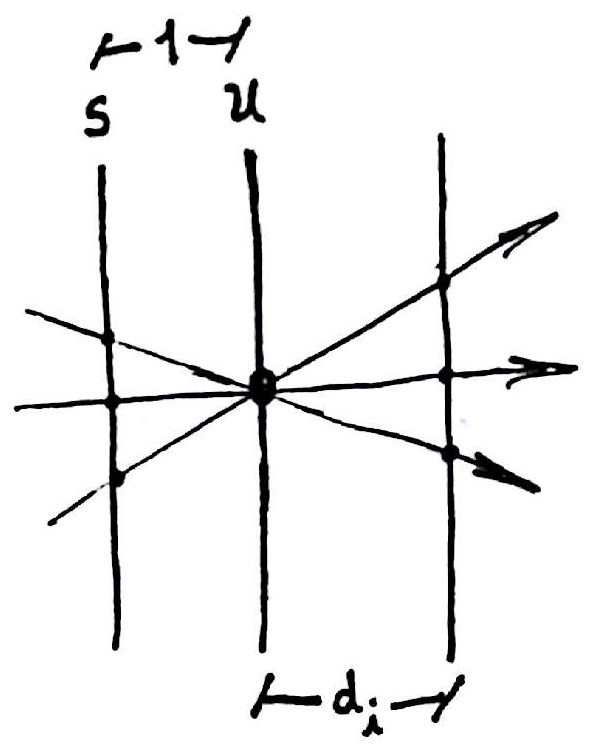
\includegraphics[height=1in]{figures/pinhole}
    \caption{Pinhole camera}\label{fig:pinhole}
  \end{subfigure}
  \quad
  \begin{subfigure}[t]{1in}
    \centering
    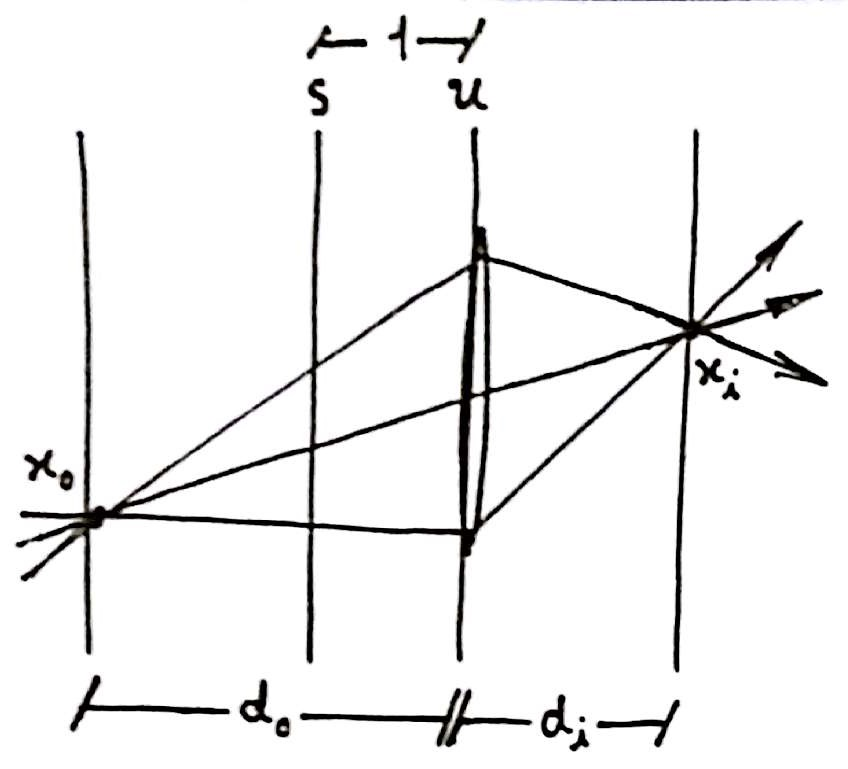
\includegraphics[height=1in]{figures/thinlens}
    \caption{Thin lens camera}\label{fig:thinlens}
  \end{subfigure}
  \caption{Camera models}\label{fig:observer}
\end{figure}

\subsection{Pinhole camera}

For a pinhole camera model, the rays intersecting the observer image plane are the rays with $u = 0$ (figure \ref{fig:pinhole}). The point with coordinate $x_{i}$ on the image plane receives a single ray described as $l(x_{i}/d_{i}, 0)$. Therefore, the frequency $\omega_{i}$ on the image plane is related to the spatial frequency by $\omega_{i} = \omega_{s}/d_{i}$.

\subsection{Thin lens camera}

For a thin lens camera model, the lens will be giving focus to a plane at an arbitrary distance $d_{o}$ (figure \ref{fig:thinlens}). The coordinate $x_{i}$ on the image plane will correspond to $x_{o} = \frac{d_{o}}{d_{i}}x_{i}$ on the plane at focus. All rays radiating from $x_{o}$ will be integrated over the angular coordinate (where the lens is located) in order to determine the pixel value in the sensor. On the frequency domain this correspond to a slice of the light field spectrum closely related to the spectrum of a Lambertian plane as described in subsection \ref{subsec:lambsurf} at a distance $d_{o}$. Likewise, $\omega_{u} = (\frac{1}{d_{o}} - 1)\omega_{s}$ and $\omega_{s} = d_{o}\omega_{o}$.

From the correspondence between $x_{o}$ and $x_{i}$ we have $\omega_{o} = \frac{d_{i}}{d_{o}}\omega_{i}$ and thereby $\omega_{i} = \omega_{s}/d_{i}$ (like the pinhole camera model). Even though the slope of the slice depends on the distance $d_{o}$, the frequency $\omega_{i}$ in the image does not.

In practice, the lens has a finite apperture that imposes bounds on the integration over the angular coordinate. Instead of dealing with those bonds directly in the integral, we can keep integrating over the entire angular plane by multiplying beforehand the light field by a $box$ filter defined solely by the angular coordinate. This multiplication corresponds to a convolution with a $sinc$ filter on the angular component of the frequency, keeping in this way the spatial frequency $\omega_{s}$, and ergo the frequency on the image $\omega_{i}$, still independent from the distance $d_{o}$.

\subsection{Discrete image}

The final discrete image is a sampling of the continuous image signal reaching the sensor. The image sampling rate determines by Nyquist-Shannon theorem the maximum frequency $\xi_{i}$ which can be represented without aliasing.

Regardless of the camera model, $\omega_{i} = \omega_{s}/d_{i}$ implies that a spatial frequency above $\xi_{s} = d_{i}\xi_{i}$ results in aliasing. Therefore, we assume that the light field does not contain spatial frequencies above $\xi_{s}$ or that it was prefiltered accordingly.

This restriction combined with the bounded Lambertian scene restrictions from subsection \ref{subsec:scene} turns the light field spectrum bandlimited (figure \ref{fig:bandlimited}).

Regarding the 4d light field, if the 2d image is sampled in a rectangular lattice (like a camera), then the horizontal and vertical spatial frequency bounds are seperable and the 4d light field spectrum is the product of two separate 2d light field spectrum as described. On the other hand, if the 2d image is sampled in a hexagonal lattice (like the human eye), the spatial frequency bounds are not seperable and neighter is the 4d light field spectrum. Even so, the light field spectrum is still bandlimited.

\begin{figure}[h]
  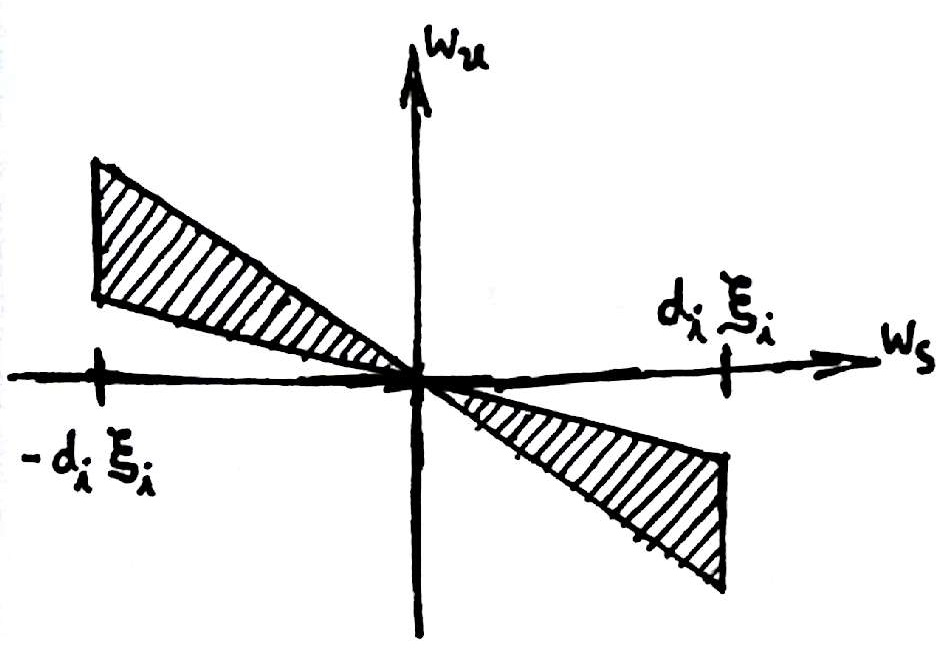
\includegraphics[height=1in]{figures/bandlimited}
  \caption{Bandlimited light field}
  \label{fig:bandlimited}
\end{figure}

\section{Sampling and filtering}

From the light field spectral analysis, different light field sampling strategies can be employed. In this section we review three strategies and their corresponding reconstruction kernels.

\subsection{Naive box filter}

The most straightforward approach is to sample the scene in a rectangular lattice over the angular and spatial coordinates. In order to prevent aliasing, the sampling rates needs to be so that the light field spectrum can be reconstructed by a box filter as in figure \ref{fig:naive}.

\begin{figure}[h]
  \centering
  \begin{subfigure}[t]{1in}
    \centering
    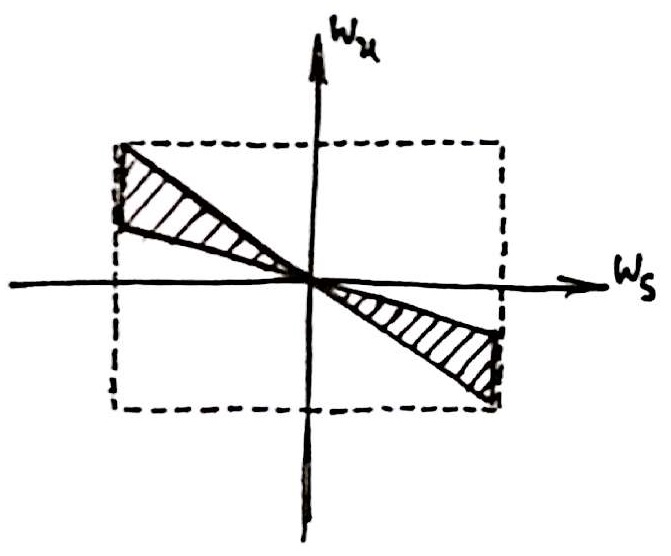
\includegraphics[width=1in]{figures/naivefilter}
    \caption{Filter}\label{fig:naivefilter}
  \end{subfigure}
  \quad
  \begin{subfigure}[t]{1in}
    \centering
    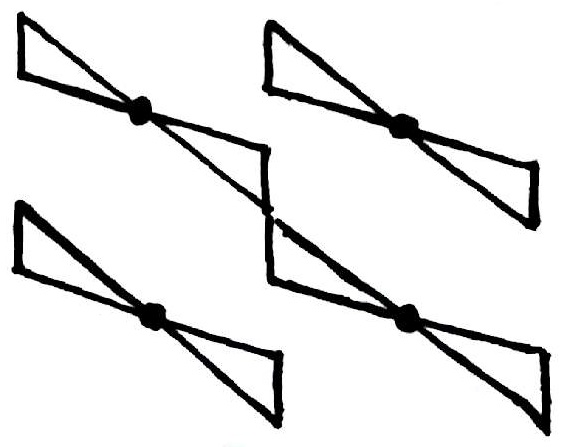
\includegraphics[width=1in]{figures/naiverep}
    \caption{Spectrum replicas}\label{fig:naiverep}
  \end{subfigure}
  \caption{Naive box filter}\label{fig:naive}
\end{figure}

\subsection{Optimum box filter}

As proposed by \cite{Chai:2000:PS:344779.344932}, the sampling rates can be reduced by changing the plane over which the sampling is done instead of the spatial plane. The optimal sampling rate is achieved for a plane at a distance $d_{m} = \frac{2}{\frac{1}{d_{min}} + \frac{1}{d_{max}}}$. The box filter over the angular frequency $\omega_{u}$ and the frequency on the sampling plane $\omega_{m}$ (figure \ref{fig:optfilter2}) is sheared over the coordinates $\omega_{u}$ and $\omega_{s}$ (figure \ref{fig:optfilter}) giving a more compact selection of the spectrum and allowing the spectrum replicas to be closer together (figures \ref{fig:optrep} and \ref{fig:optrep2}).

\begin{figure}[h]
  \centering
  \begin{subfigure}[t]{1in}
    \centering
    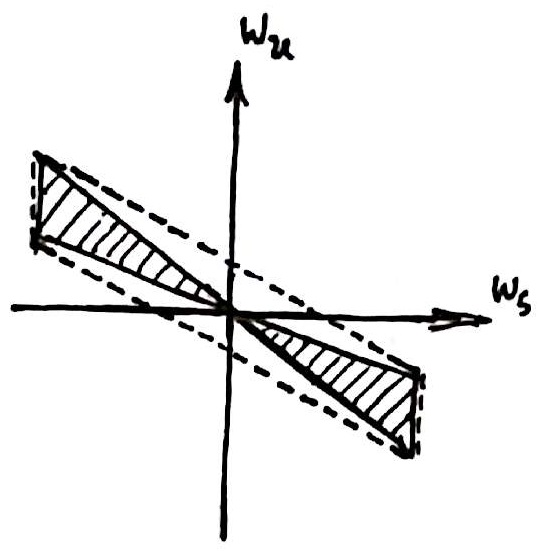
\includegraphics[width=1in]{figures/optfilter}
    \caption{Filter}\label{fig:optfilter}
  \end{subfigure}
  \quad
  \begin{subfigure}[t]{1in}
    \centering
    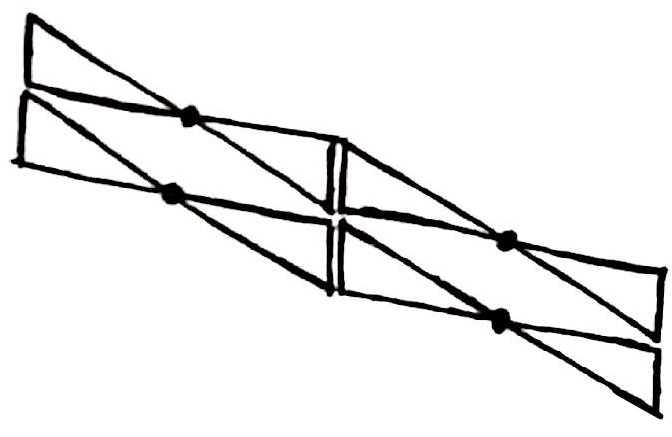
\includegraphics[width=1in]{figures/optrep}
    \caption{Spectrum replicas}\label{fig:optrep}
  \end{subfigure}
  \caption{Optimum box filter (light field coordinates)}\label{fig:opt}
\end{figure}

\begin{figure}[h]
  \centering
  \begin{subfigure}[t]{1in}
    \centering
    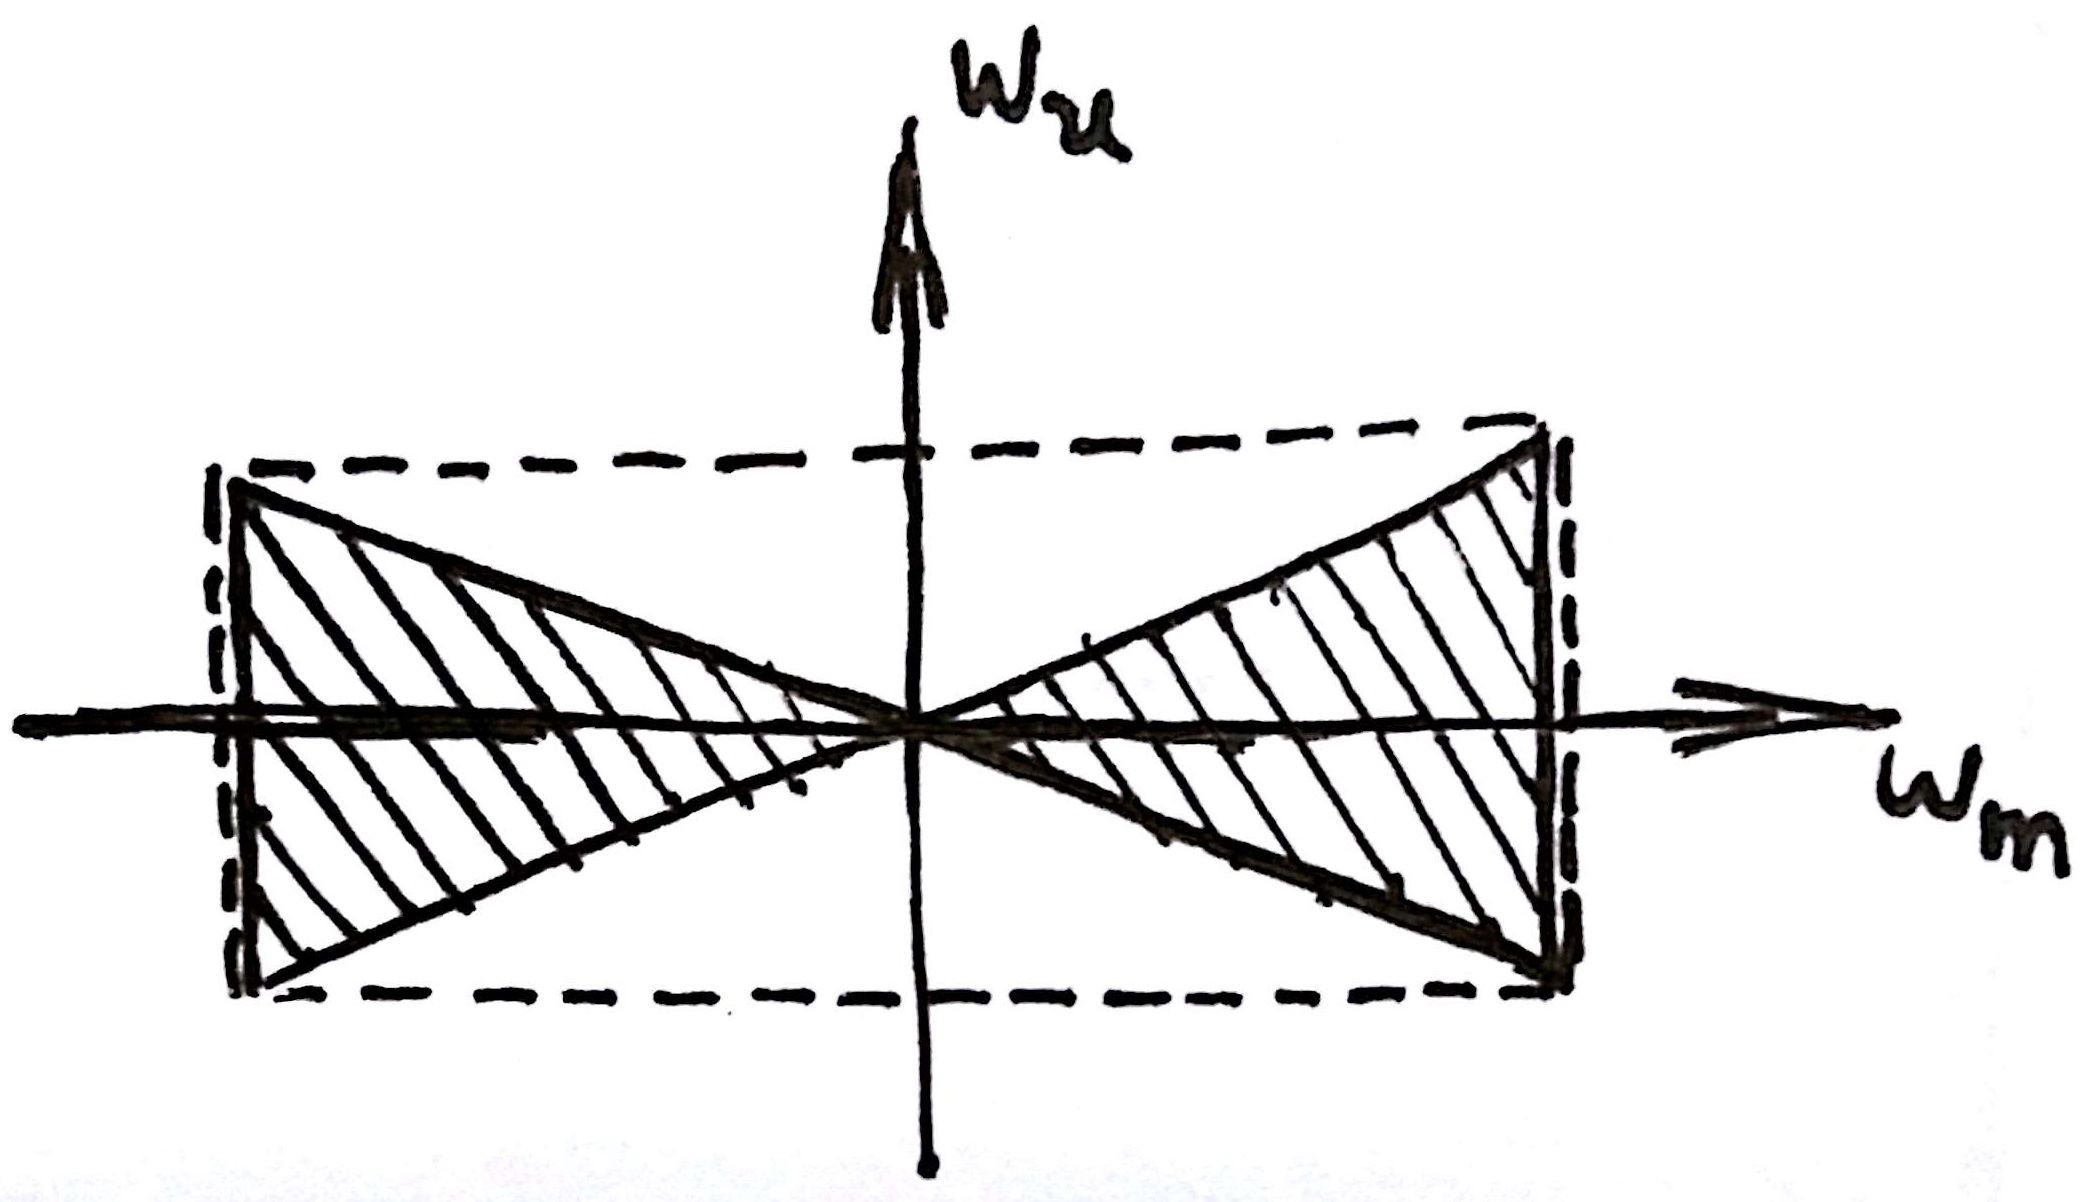
\includegraphics[width=1in]{figures/optfilter2}
    \caption{Filter}\label{fig:optfilter2}
  \end{subfigure}
  \quad
  \begin{subfigure}[t]{1in}
    \centering
    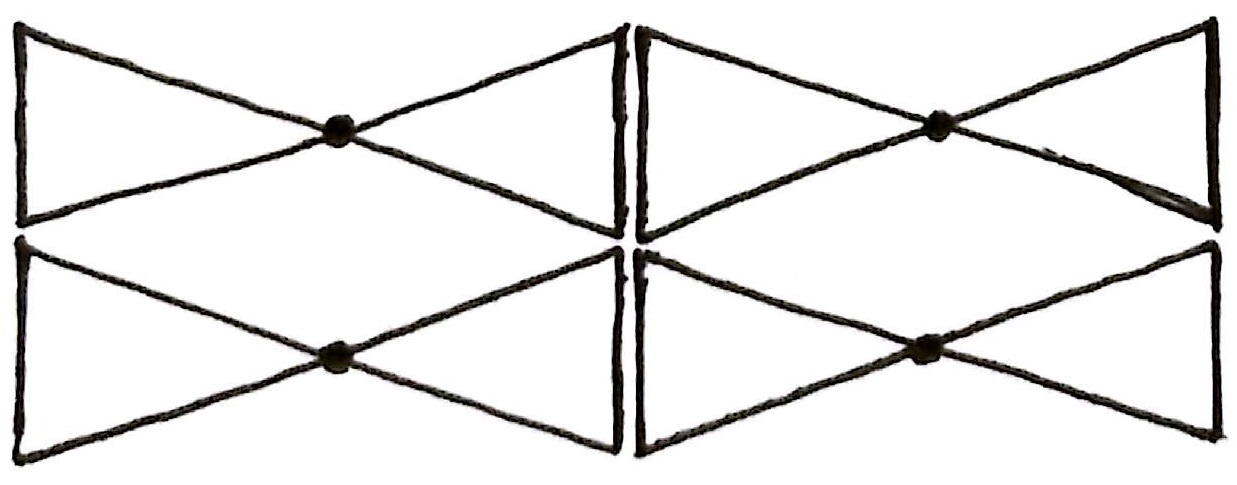
\includegraphics[width=1in]{figures/optrep2}
    \caption{Spectrum replicas}\label{fig:optrep2}
  \end{subfigure}
  \caption{Optimum box filter (sampling coordinates)}\label{fig:opt2}
\end{figure}

\subsection{Optimum arbitrary shape filter}

The spectrum replicas can be arranged even closer together, covering all the frequency domain without any gaps (figures \ref{fig:fanrep} and \ref{fig:fanrep2}). In this arrangement the signal can not be reconstructed with a box filter. A custom filter needs to be designed to match the exact shape of the spectrum (figures \ref{fig:fanfilter} and \ref{fig:fanfilter2}) as proposed by \cite{zhang2001generalized}. Nonetheless, the sampling is still rectangular (figure \ref{fig:fanrep2}) for the right coordinates, in this case over the planes at distances $d_{min}$ and $d_{max}$.

\begin{figure}[h]
  \centering
  \begin{subfigure}[t]{1in}
    \centering
    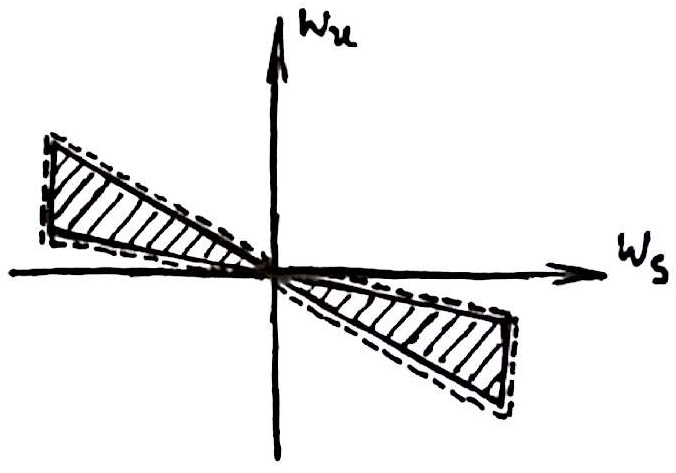
\includegraphics[width=1in]{figures/fanfilter}
    \caption{Filter}\label{fig:fanfilter}
  \end{subfigure}
  \quad
  \begin{subfigure}[t]{1in}
    \centering
    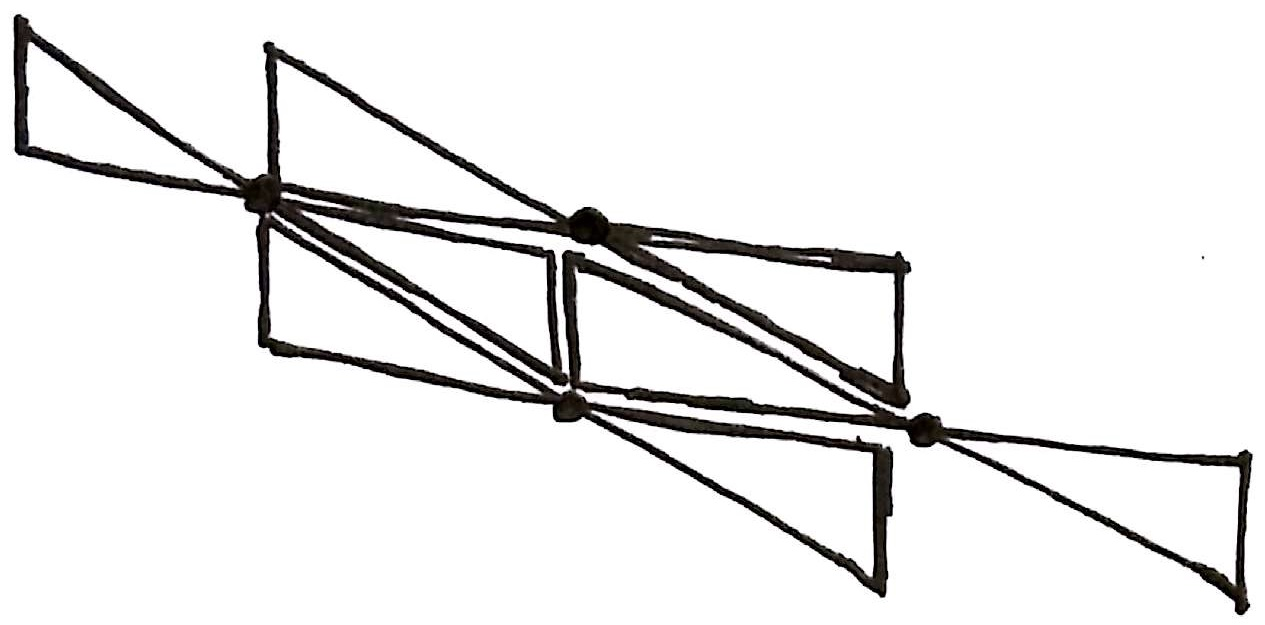
\includegraphics[width=1in]{figures/fanrep}
    \caption{Spectrum replicas}\label{fig:fanrep}
  \end{subfigure}
  \caption{Optimum arbitrary shape filter (light field coordinates)}\label{fig:fan}
\end{figure}

\begin{figure}[h]
  \centering
  \begin{subfigure}[t]{1in}
    \centering
    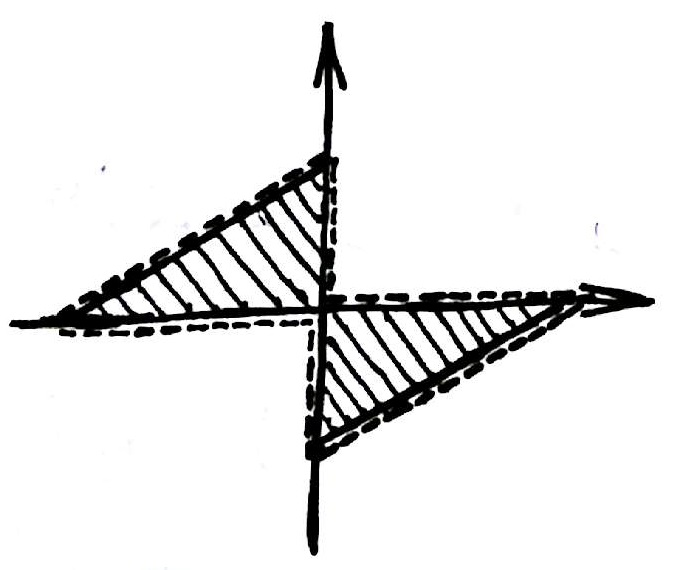
\includegraphics[width=1in]{figures/fanfilter2}
    \caption{Filter}\label{fig:fanfilter2}
  \end{subfigure}
  \quad
  \begin{subfigure}[t]{1in}
    \centering
    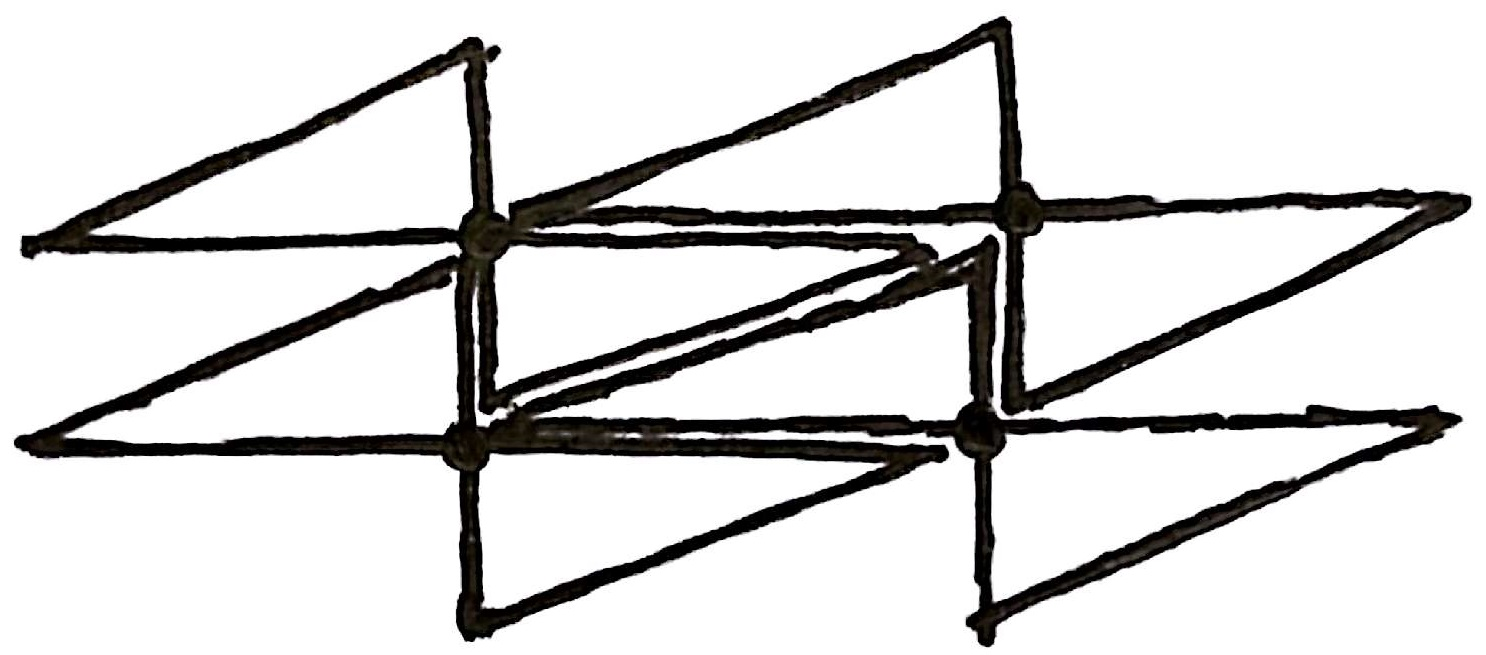
\includegraphics[width=1in]{figures/fanrep2}
    \caption{Spectrum replicas}\label{fig:fanrep2}
  \end{subfigure}
  \caption{Optimum arbitrary shape filter (sampling coordinates)}\label{fig:fan2}
\end{figure}

\section{Dual-layer automultiscopic display}

\cite{Lanman:2010:CPB:1882261.1866164}

A new family of compressive light field displays called tensor displays was introduced by \cite{Wetzstein:2012:TDC:2185520.2185576}. Multiple layers of LCD panels are stacked, each atenuating the rays emited by a backlight. The

\subsection{Multiplicative modulation}
\subsection{Non-negative factorization}
\subsection{Time-multiplexing}
\subsection{The light field stereoscope}
\subsection{Ray interpolation/integration}

\section{Experiments}

\section{Conclusion and future work}

Conclusion...

\bibliographystyle{ACM-Reference-Format}
\bibliography{bibliografia}

\end{document}
